
% !TEX root = ../FundationsDataScience.tex

\chapter{Theory of Sparse Regularization}

We now apply the basics elements of convex analysis from the previous chapter to perform a theoretical analysis of the properties of the Lasso, in particular its performances to recover sparse vectors.





%%%%%%%%%%%%%%%%%%%%%%%%%%%%%%%%%%%%%%%%%%%%%%%%%%%%%%%%%%%%%%%%%%%%%%%%%%%%%%%%%%
%%%%%%%%%%%%%%%%%%%%%%%%%%%%%%%%%%%%%%%%%%%%%%%%%%%%%%%%%%%%%%%%%%%%%%%%%%%%%%%%%%
%%%%%%%%%%%%%%%%%%%%%%%%%%%%%%%%%%%%%%%%%%%%%%%%%%%%%%%%%%%%%%%%%%%%%%%%%%%%%%%%%%
\section{Existence and Uniqueness}


%%%%%%%%%%%%%%%%%%%%%%%%%%%%%%%%%%%%%%%%%%%%%%%%%%%%%%%%%%%%%%%%%%%%%%%%%%%%%%%%%%
\subsection{Existence}

We consider problems~\eqref{eq-lasso-lagr-ip} and~\eqref{eq-lasso-constr-ip}, that we rewrite here as 
\eql{\label{eq-lasso-lagr}\tag{$\Pp_\la(y)$}
	\umin{x \in \RR^N} f_\la(x) \eqdef \frac{1}{2\la} \norm{y-Ax}^2 + \la \norm{x}_1
} 
and its limit as $\la \rightarrow 0$
\eql{\label{eq-lasso-constr}\tag{$\Pp_0(y)$}
	\umin{A x = y} \norm{x}_1
	= \umin{x} f_0(x) \eqdef \iota_{\Ll_y}(x) + \norm{x}_1.
} 
where $A \in \RR^{P \times N}$, and $\Ll_y \eqdef \enscond{x \in \RR^N}{Ax=y}$.

We recall that the setup is that one observe noise measures
\eq{
	y=A x_0 + w
}
and we would like conditions to ensure for $x_0$ to solution to $(\Pp_0(Ax_0))$ (i.e. when $w=0$) and to be close (in some sense to be defined, and in some proportion to the noise level $\norm{w}$) to the solutions of $(\Pp_0(y=Ax_0+w))$ when $\la$ is wisely chosen as a function of $\norm{w}$. 

First let us note that since~\eqref{eq-lasso-lagr} is unconstrained and coercive (because $\norm{\cdot}_1$ is), this problem always has solutions.
%
Since $A$ might have a kernel and $\norm{\cdot}_1$ is not strongly convex, it might have non-unique solutions.
%
If $y \in \Im(A)$, the constraint set of~\eqref{eq-lasso-constr} is non-empty, and it also has solutions, which might fail to be unique.



\begin{figure}
\centering
%%
\begin{tabular}{@{}c@{}c@{}}
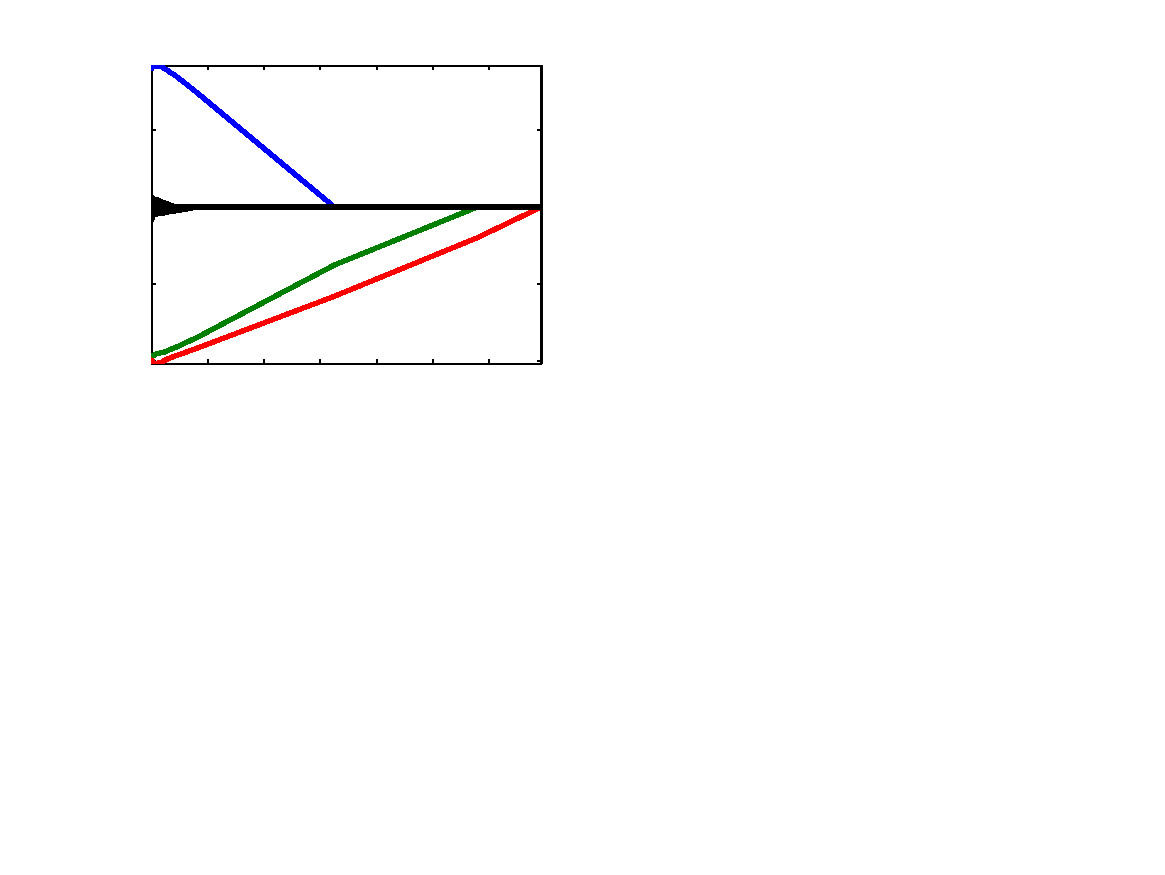
\includegraphics[width=.35\linewidth]{sparse-theory/homotopy/homotopy-s3}&
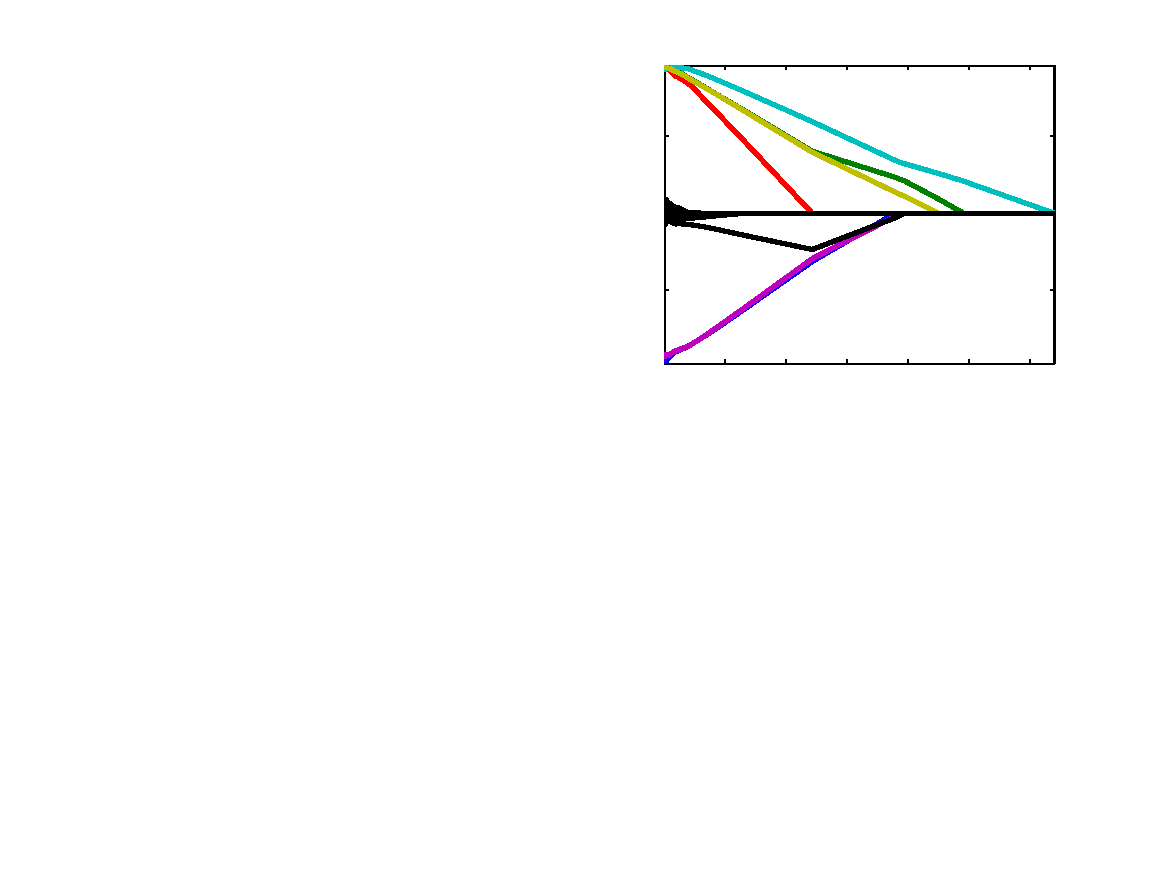
\includegraphics[width=.35\linewidth]{sparse-theory/homotopy/homotopy-s6}\\
$s=3$  & $s=6$ \\
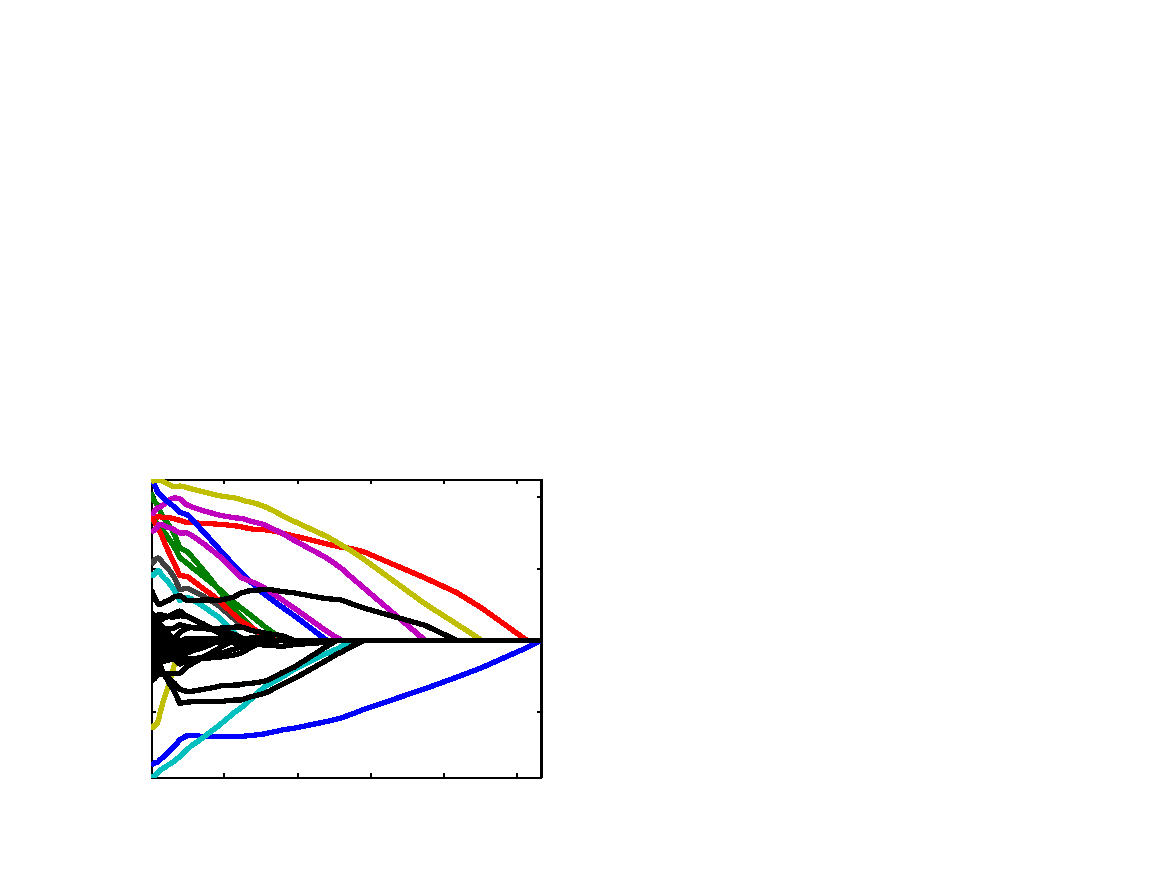
\includegraphics[width=.35\linewidth]{sparse-theory/homotopy/homotopy-s13}&
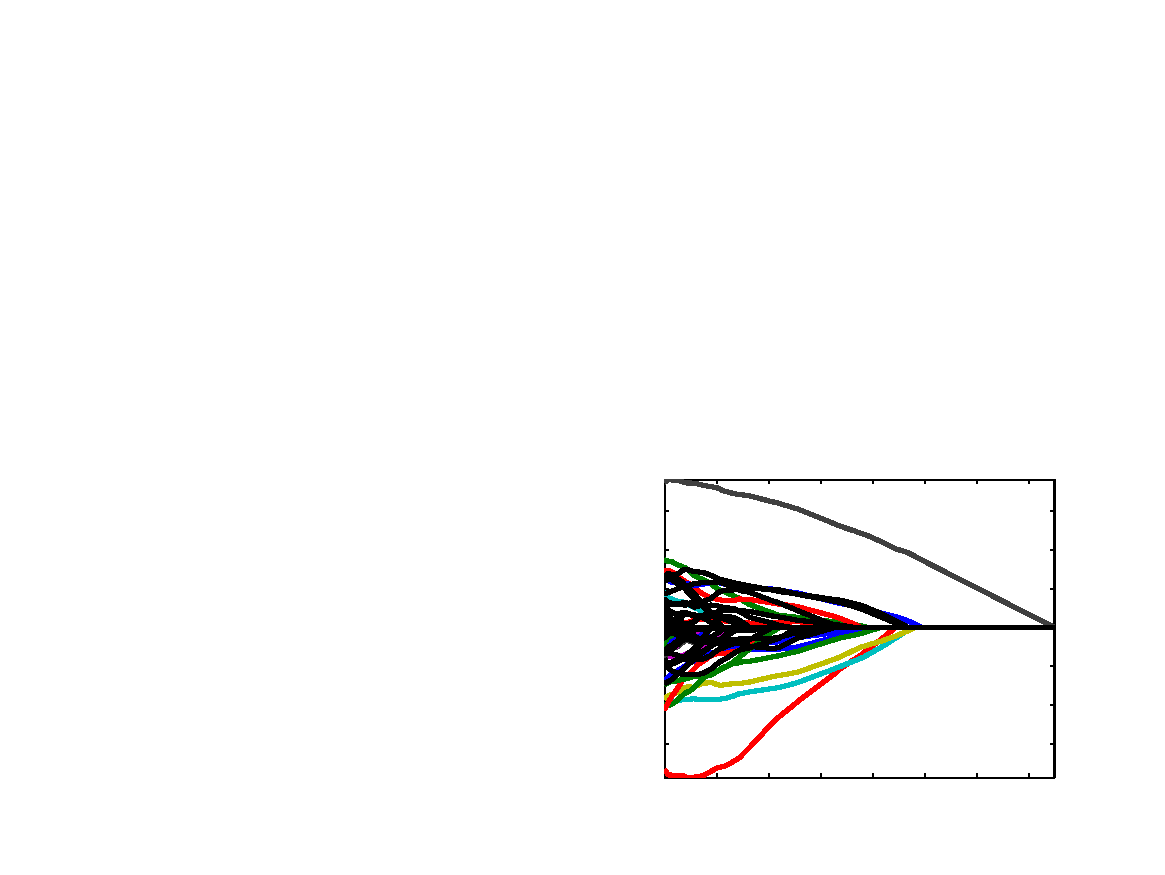
\includegraphics[width=.35\linewidth]{sparse-theory/homotopy/homotopy-s25}\\
$s=13$  & $s=25$ 
\end{tabular}
%%
\caption{\label{fig-homotopy}
Display of the evolution $\la \mapsto x_\la$ of the solutions of~\eqref{eq-lasso-lagr}.
}
\end{figure}

Figure~\ref{fig-homotopy} gives the intuition of the theory that will be developed in this chapter, regarding the exact or approximated recovery of sparse vectors $x_0$, and the need for a careful selection of the $\la$ parameter.





%%%%%%%%%%%%%%%%%%%%%%%%%%%%%%%%%%%%%%%%%%%%%%%%%%%%%%%%%%%%%%%%%%%%%%%%%%%%%%%%%%
\subsection{Polytope Projection for the Constraint Problem}
\label{sec-polytope-proj}

The following proposition gives a geometric description of those vectors which are recovered by $\ell^1$ minimization when there is no noise. 

\begin{prop}\label{prop-polytope-proj}
	We denote $B \eqdef \enscond{x \in \RR^N}{\norm{x}_1 \leq 1}$. Then
	\eql{\label{eq-polytop-ident} 
		x_0 \text{ is a solution to } \Pp_0(Ax_0)
		\quad\Longleftrightarrow\quad
		A \frac{x_0}{\norm{x_0}_1} \in \partial (AB)
	} 
	where ``$\partial$'' denoted the boundary and $AB=\enscond{Ax}{x\in B}$.
\end{prop}
\begin{proof}
	We first prove $``\Rightarrow''$. We suppose that $x_0$ is not a solution, and aim at showing that $A \frac{x_0}{\norm{x_0}_1} \in \text{int}(AB_\rho)$. Since it is not a solution, there exists $z$ such that $Ax_0=Az$ and $\norm{z}_1 = (1-\de)\norm{x_0}_1$ with $\de>0$. Then for any displacement $h=A\epsilon \in \Im(A)$, one has $Ax_0+h=A(z+\epsilon)$ and
	\eq{
		\norm{z+\epsilon}_1 \leq \norm{z}_1 + \norm{\Phi^+ h} \leq (1-\de) \norm{x_0}_1 + \norm{\Phi^+}_{1,1} \norm{h}_1 < \frac{\de}{\norm{A^+}_{1,1}}\norm{x_0}.
	}
	This means that choosing $\norm{h}_1 < \frac{\de}{\norm{A^+}_{1,1}} \norm{x_0}_1$ implies that $A \frac{x_0}{\norm{x_0}_1} \in \text{int}(AB)$.
	
	We now prove ``$\Leftarrow$''. We suppose that $A \frac{x_0}{\norm{x_0}_1} \in \text{int}(AB)$. Then there exists $z$ such that $Ax_0=(1-\de) Az$ and $\norm{z}_1 < \norm{x_0}_1$. This implies $\norm{(1-\de)z}_1 < \norm{x_0}_1$ so that $(1-\de)z$ is better than $x_0$ which is thus not a solution. 
\end{proof}

This results state that ``friendly'' identifiable vectors (those recovered by $\ell^1$) are those who gets projected by $A$ on the boundary of the polytope $\norm{x_0}_1 A B$. Intuitively, if $P$ is small in comparison to $N$, then this projected polytope is small, and most vector will failed to be reconstructed by solving $\ell^1$ minimization. This also suggests why using random projections as in Chapter~\ref{chap-cs}, because somehow they results in a low distortion embedding of the $\ell^1$ ball from $\RR^N$ to $\RR^P$.

Note that if $x_0$ is identifiable, so is $\la x_0$ for $\rho x_0$ for $\rho>0$, and in fact, since the recovery condition only depends on the geometry of the faces of $B$, the obtained condition~\eqref{eq-polytop-ident} only depends on $\sign(x_0)$. 
%
We denote $\Aa : y \mapsto x^\star$ the map from $y$ to a solution of~\eqref{eq-lasso-constr}, which we assume is unique for simplicity of exposition.
%
Condition~\eqref{eq-polytop-ident} thus shows that $A$ and $\Aa$ are inverse bijection on a family of cones $\Cc_s = \enscond{x}{\sign(x)=s}$ and $A\Cc_s$ for certain ``friendly'' sign patterns $s$. These cones $A\Cc_s$ form a partition of the image space $\RR^P$. Assuming for simplicity that the columns $(a_j)_j$ of $A$ have unit norm, for $P=3$, the interaction of these $A\Cc_s$ with the unit sphere of $\RR^3$ for a so-called Delaunay triangulation of the sphere (this construction extends to higher dimension by replacing triangle by simplexes), see also Figure~\ref{fig-delaunay}. Such Delaunay triangulation is characterized by the empty spherical cap property (each circumcircle associated to a triangle should not contains any columns vector $a_j$ of the matrix).
%
Figure~\ref{fig-polytopes} illustrate these conclusions in $\RR^2$ and $\RR^3$. 


\begin{figure}
\centering
%%
\begin{tabular}{@{}c@{}c@{\hspace{3mm}}c@{}}
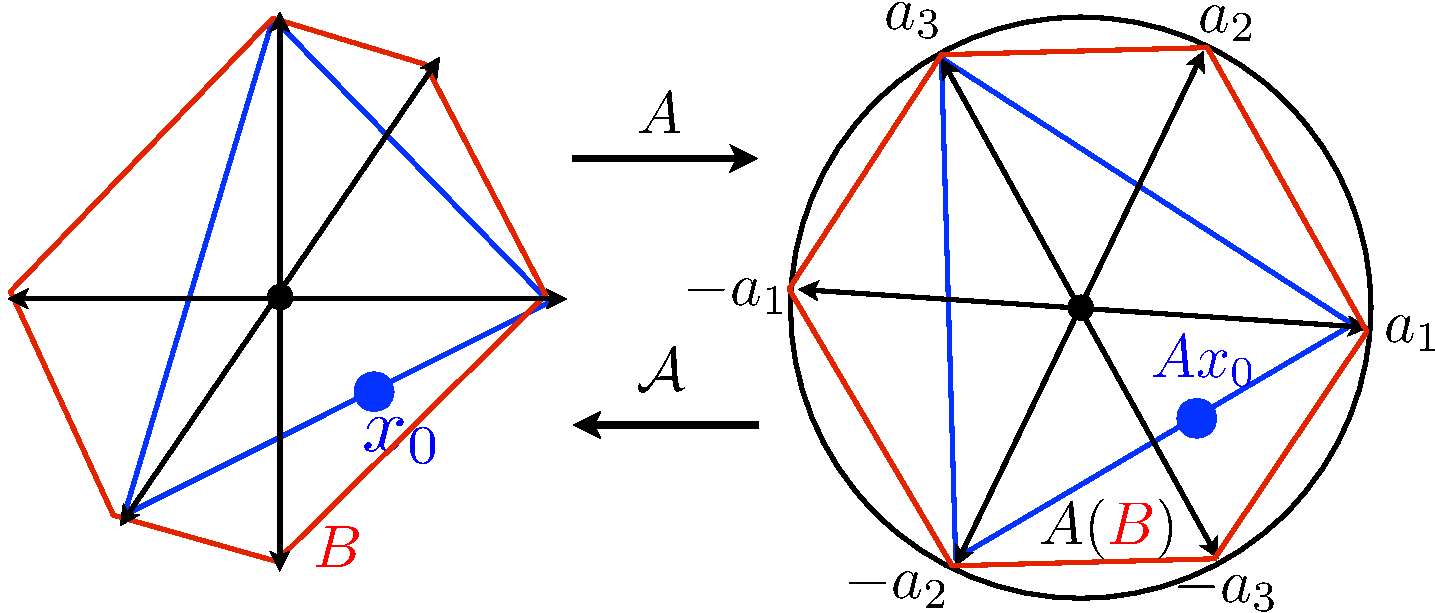
\includegraphics[width=.35\linewidth]{sparse-theory/polytopes/polytopes-32-1}&
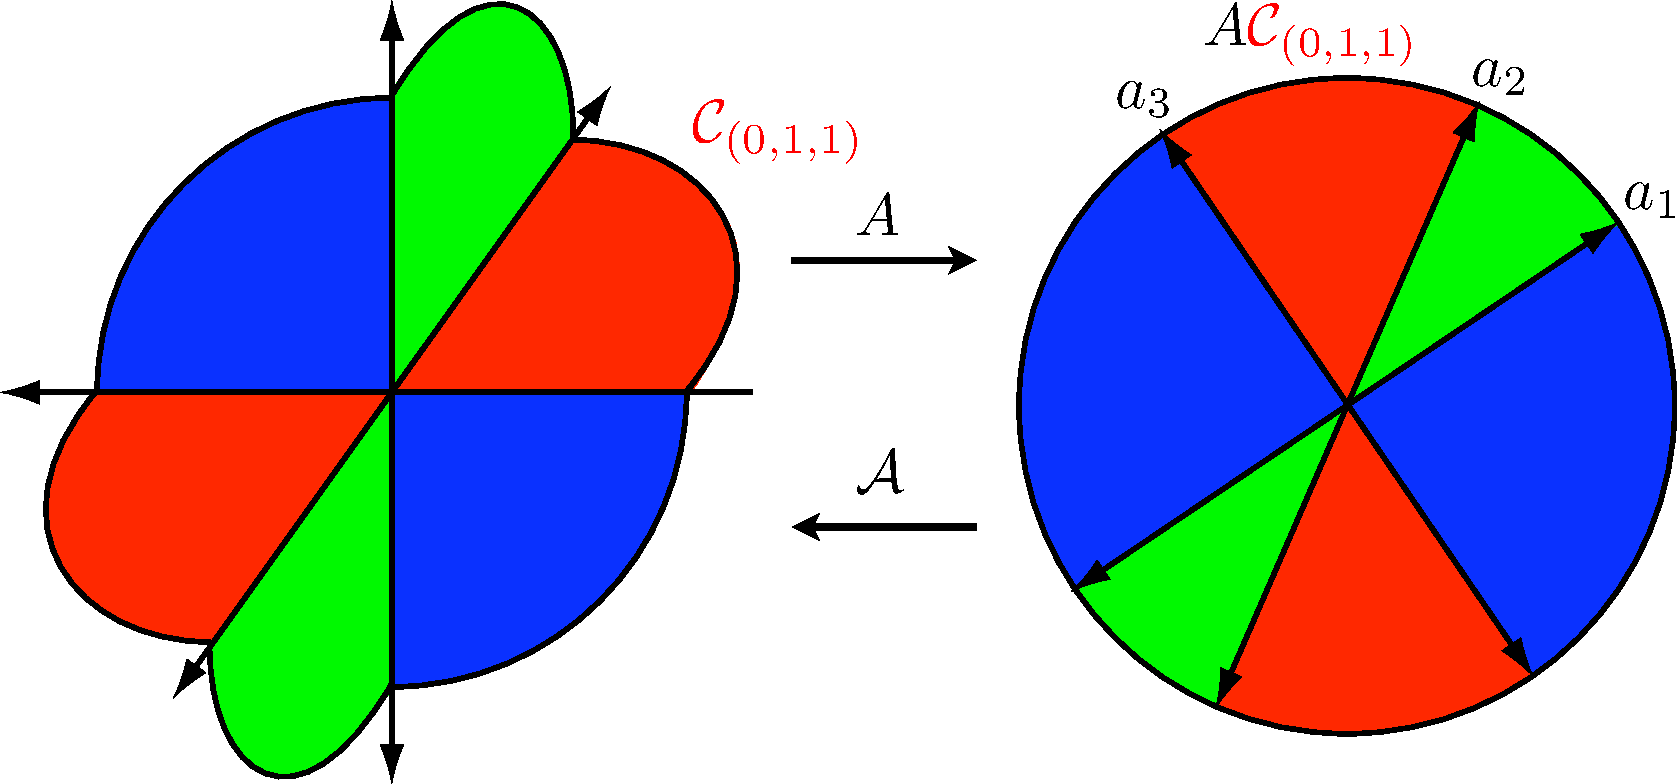
\includegraphics[width=.35\linewidth]{sparse-theory/polytopes/polytopes-32-2}&
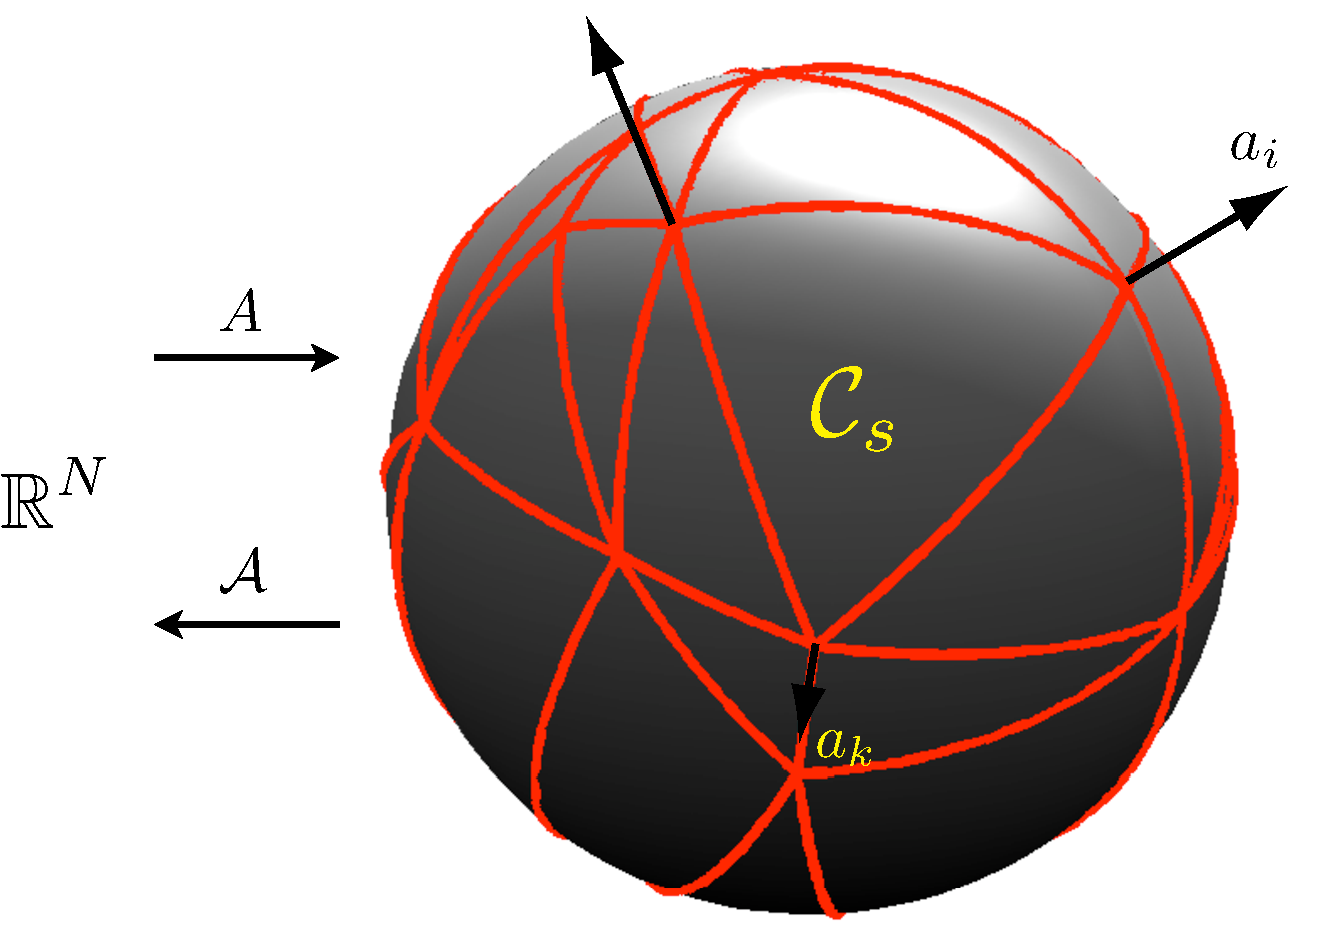
\includegraphics[width=.25\linewidth]{sparse-theory/polytopes/polytopes-3d}\\
$A\in \RR^{2\times 3}$& $A\in \RR^{2\times 3}$ & $A\in \RR^{3\times N}$
\end{tabular}
%%
\caption{\label{fig-polytopes}
Display of the action of the linear map $A$ on the $\ell^1$ ball $B$, and of the inverse non-linear map $\Aa$ defined by the solution of~\eqref{eq-lasso-constr}. 
}
\end{figure}

%%%%%%%%%%%%%%%%%%%%%%%%%%%%%%%%%%%%%%%%%%%%%%%%%%%%%%%%%%%%%%%%%%%%%%%%%%%%%%%%%%
\subsection{Optimality Conditions}

In the following, given an index set $I \subset \{1,\ldots,N\}$, denoting $A=(a_i)_{i=1}^N$ the columns of $A$, we denote $A_I \eqdef (a_i)_{i \in I} \in \RR^{P \times |I|}$ the extracted sub-matrix.  Similarly, for $x \in \RR^N$, we denote $x_I \eqdef (x_i)_{i \in I} \in \RR^{|I|}$. 

The following proposition rephrases the first order optimality conditions in a handy way. 

\begin{prop}\label{prop-first-order-lagr}
	$x_\la$ is a solution to~\eqref{eq-lasso-lagr} for $\la>0$ if and only if
	\eq{
		\eta_{\la,I} = \sign(x_{\la,I})
		\qandq
		\norm{\eta_{\la,I^c}} \leq \la
	}
	where we define
	\eql{\label{eq-defn-eta-lamb}
		I\eqdef \supp(x_\la) \eqdef \enscond{i}{ x_{\la,i} \neq 0 }, 
		\qandq	\eta_\la \eqdef \frac{1}{\la}A^*(y-Ax_\la).
	}
\end{prop}
\begin{proof}
Since~\eqref{eq-lasso-lagr} involves a sum of a smooth and a continuous function, its sub-differential reads
\eq{
	\partial f_\la(x) = \frac{1}{\la}A^*(Ax-y) + \la\partial\norm{\cdot}_1(x).
} 
Thus $x_\la$ is solution to~\eqref{eq-lasso-lagr} if and only if $0 \in \partial f_\la(x_\la)$, which gives the desired result. 
\end{proof}

The following proposition studies the limit case $\la=0$ and introduces the crucial concept of ``dual certificates'', which are the Lagrange multipliers of the constraint $\Ll_y$.

\begin{prop}\label{prop-first-order-constr}
	$x^\star$ being a solution to~\eqref{eq-lasso-constr} is equivalent to having $Ax^\star=y$ and that
	\eql{\label{eq-defn-dual-certif}
		\exists \eta \in \Dd_0(y,x^\star) \eqdef \Im(A^*) \cap \partial \norm{\cdot}_1(x^\star).
	}
\end{prop}
\begin{proof}
Since~\eqref{eq-lasso-constr} involves a sum with a continuous function, one can also computes it sub-differential as
\eq{
	\partial f_0(x) = \partial \iota_{\Ll_y}(x) + \partial\norm{\cdot}_1(x).
}
If $x \in \Ll_y$, then $\partial \iota_{\Ll_y}(x)$ is the linear space orthogonal to $\Ll_y$, i.e. $\ker(A)^\bot=\Im(A^*)$. 
\end{proof}

Writing $I=\supp(x^\star)$, one thus has
\eq{
	\Dd_0(y,x^\star) = \enscond{ \eta = A^* p }{
		\eta_I = \sign(x^\star_I), \:
		\norm{\eta}_\infty \leq 1
	}.
}
Although it looks like the definition of $\Dd_0(y,x^\star)$ depends on the choice of a solution $x^\star$, convex duality (studied in the next chapter) shows that it is not the case (it is the same set for all solutions).

%%%%%%%%%%%%%%%%%%%%%%%%%%%%%%%%%%%%%%%%%%%%%%%%%%%%%%%%%%%%%%%%%%%%%%%%%%%%%%%%%%
\subsection{Uniqueness}

The following proposition shows that the Lasso selects a set of linearly independent regressors (columns of $A$). This is why this method is also often called ``basis pursuit''. 

\begin{prop}
	For $\la \geq 0$, there is always a solution $x^\star$ to~\eqref{eq-lasso-lagr} with $I=\supp(x^\star)$ such that $\ker(A_I)=\{0\}$
\end{prop}
\begin{proof}
	Let $x$ be a solution and denote $I=\supp(x)$.
	%
	If $\ker(A_I) \neq \{0\}$, one selects $h_I \in \ker(A_I)$ and define for $t \in \RR$ the vector $x_t \eqdef x+th$.
	We denote $t_0$ the smallest $|t|$ such that $\sign(x_t) \neq \sign(x)$, i.e. $\supp(x_t)$ is strictly included in $I$.
	%
	For $t<t_0$, since $Ax_t=Ax$ and $\sign(x_t)=\sign(x)$, $x_t$ still satisfies the same first order condition as $x_0$, and one can apply  either Proposition~\ref{prop-first-order-constr} (for $\la=0$) or Proposition~\ref{prop-first-order-lagr} (for $\la>0$), so that $x_t$ is a solution of~\eqref{eq-lasso-lagr}.
	%
	Since the minimized function are lower semi continuous, $x_t \rightarrow x_{t_0}$ is still a solution.
	%
	If $\ker(A_{J}) \neq \{0\}$ with $J=\supp(x_{t_0})$, one is over, otherwise one can iterate this argument on $x_{t_0}$ in place of $x$ and have a  sequence of supports which is strictly decaying in size, so it must terminate. 
\end{proof}

This results in particular that if columns of $A_I$ are not independent, then the solution of~\eqref{eq-lasso-lagr} is necessarily non-unique. 

Assuming that $x_\la$ is a solution such that $\ker(A_I)=\{0\}$, then from~\eqref{eq-lasso-lagr},  one obtains the following implicit expression for the solution
\eql{\label{eq-local-shape-lasso}
	x_{\la,I} = A_I^+ y - \la (A_I^*A_I)^{-1} \sign(x_{\la,I}).
}
This expression can be understood as a form of generalized soft thresholding (one retrieve the soft thresholding when $A=\Id_N$). 

The following useful lemma shows that while solutions $x_\la$ to~\eqref{eq-lasso-lagr} are not necessarily unique, the associated ``predictor'' (i.e. denoised version of $y$) $Ax_\la$ is however always uniquely defined.    
%
Note that according to~\eqref{eq-local-shape-lasso}, one has 
\eql{\label{eq-local-shape-lasso}
	\Phi x_{\la} = \Proj_{\Im(A_I)} y - \la A_I (A_I^*A_I)^{-1} \sign(x_{\la,I}).
}
so up to a $O(\la)$ bias, this predictor is an orthogonal projection on a low dimensional subspace indexed by $I$. 


\begin{lem}\label{lem-unique-predict}
	For $\la \geq 0$, if $(x_1,x_2)$ are solution to~\eqref{eq-lasso-lagr}, then $Ax_1=Ax_2$. 
\end{lem}
\begin{proof}
	For $\la=0$, this is trivial because $Ax_1=Ax_2=y$. Otherwise, let us assume $Ax_1 \neq Ax_2$. Then for $x=(x_1+x_2)/2$, one has
	\eq{
		\norm{x}_1 \leq \frac{ \norm{x_1}_1 + \norm{x_2}_2 }{2}
		\qandq
		\norm{Ax-y}^2 < \frac{ \norm{Ax_1-y}^2 + \norm{Ax_2-y}^2 }{2}		
	}
	where the second inequality follows from the strict convexity of the square. This shows that
	\eq{
		\frac{1}{2\la}\norm{Ax-y}^2 +\norm{x}_1 <
		\frac{1}{2\la}\norm{Ax_1-y}^2 +\norm{x_1}_1, 
	}
	which is a contradiction to the optimality of $x_1$. 
\end{proof}


\begin{prop}\label{sec-prop-uniquness-lagr}
 	Let $x_\la$ be a solution to~\eqref{eq-lasso-lagr} and denote $\eta_\la \eqdef \frac{1}{\la}A^*(y-A x_\la)$.
	%
	We define the ``extended support'' as 
	\eq{
		J \eqdef \sat(\eta_\la) \eqdef \enscond{i}{|\eta_{\la,i}|=1}.
	}
	If $\ker(A_{J})=\{0\}$ then $x_\la$ is the unique solution of~\eqref{eq-lasso-lagr}.
\end{prop}
\begin{proof}
	If $\tilde x_\la$ is also a minimizer, then by Lemma~\ref{lem-unique-predict}, 
	$Ax_\la=A\tilde x_\la$, so that in particular they share the same dual certificate
	\eq{
		\eta_\la = \frac{1}{\la}A^*(y-Ax_\la) = \frac{1}{\la}A^*(y-A\tilde x_\la).
	}
	The first order condition, Proposition~\ref{prop-first-order-lagr}, shows that necessarily 
	$\supp(x_\la) \subset J$ and $\supp(\tilde x_\la) \subset J$.
	%
	Since $A_J x_{\la,J} = A_J \tilde x_{\la,J}$, and since $\ker(A_J)=\{0\}$, one has 
	$x_{\la,J}=\tilde x_{\la,J}$, and thus $x_\la=\tilde x_\la$ because of their supports are included in $J$.
\end{proof}

\begin{prop}\label{sec-prop-uniquness-constr}
 	Let $x^\star$ be a solution to~\eqref{eq-lasso-constr}. If there exists $\eta \in \Dd_0(y,x^\star)$ such that 
	$\ker(A_{J})=\{0\}$ where $J \eqdef \sat(\eta)$ then $x^\star$ is the unique solution of~\eqref{eq-lasso-constr}.
\end{prop}
\begin{proof}
	The proof is the same as for Proposition~\ref{sec-prop-uniquness-lagr}, replacing $\eta_\la$ by $\eta$. 
\end{proof}

These propositions can be used to show that if $A$ is drawn according to a distribution having a density over $\RR^{p \times n}$, then with probability $1$ on the matrix $A$, the solution to~\eqref{eq-lasso-lagr} is unique. Note that this results is not true if $A$ is non random but $y$ is.



%%%%%%%%%%%%%%%%%%%%%%%%%%%%%%%%%%%%%%%%%%%%%%%%%%%%%%%%%%%%%%%%%%%%%%%%%%%%%%%%%%
\subsection{Duality}
\label{sec-duality-lasso}

We now related the first order conditions and ``dual certificate'' introduced above to the duality theory detailed in Section~\ref{sec-cvx-duality}. This is not strictly needed to derive the theory of sparse regularization, but this offers an alternative point of view and allows to better grasp the role played by the certificates. 


\begin{thm}
	For any $\la \geq 0$ (i.e. including $\la=0$), one has strong duality between~\eqref{eq-lasso-lagr} and
	\eql{\label{eq-dual-lasso}
		�\usup{p \in \RR^P} \enscond{ \dotp{y}{p} - \frac{\la}{2} \norm{p}^2 }{ \norm{A^* p}_\infty \leq 1 }.
	}
	One has for any $\la \geq 0$ that $(x^\star,p^\star)$ are primal and dual solutions if and only if
	\eql{\label{eq-pd-support-localization}
		A^* p^\star \in \partial \norm{\cdot}_1(x^\star)
		\quad\Leftrightarrow\quad
		\pa{
		I \subset \sat(A^* p)
		\qandq
		\sign(x_I^\star) = A_I^* p
		}, 
	}
	where we denoted $I=\supp(x^\star)$, 
	%
	and furthermore, for $\la>0$, 
	\eq{
		p^\star = \frac{y-A x^\star}{\la}.
	}
	while for $\la=0$, $Ax^\star=y$.
\end{thm}

\begin{proof}
	There are several ways to derive the same dual. One can for instance directly use the Fenchel-Rockafeller formula~\eqref{eq-fenchel-rockafeller}. But it is instructive to do the computations using Lagrange duality. One can first consider the following re-writing of the primal problem
	\eq{
		\umin{x \in \RR^N} \enscond{ f(z) + \norm{x}_1 }{ Ax=z } = \umin{x \in \RR^N} \usup{p \in \RR^p} \Ll(x,z,p) \eqdef f_\la(z) + \norm{x}_1 + \dotp{z-Ax}{p}
	}
	where $f_\la(z) \eqdef \frac{1}{2\la}\norm{z-y}^2$ if $\la>0$ and $f(z)=\iota_{\{y\}}(z)$ if $\la=0$.
	%
	For $\la>0$ since $f_\la$ and $\norm{\cdot}_1$ are continuous, strong duality holds. 
	%
	For $\la=0$, since the constraint appearing in $f_0$ is linear (actually a singleton), strong duality holds also. 
	%
	Thus using Theorem~\ref{thm-strong-duality}, one can exchange the min and the max and obtains
	\eq{
		\umax{p \in \RR^P}�\pa{�\min{z}�\dotp{z}{p}+ f_\la(z)  } +�\pa{ \min{x}�\norm{x}_1 - \dotp{x}{A^*p} }
		= \umax{p \in \RR^P} - f_\la^*( -p ) - (\norm{\cdot}_1)^*( A^* p ).
	}
	Using~\eqref{prop-dual-lp}, one has that $(\norm{\cdot}_1^* = \iota_{\norm{\cdot}_\infty \leq 1}$. 
	%
	For $\la>0$, one has using Proposition~\ref{eq-example-legendre} that 
	\eq{
		f_\la^* = ( \frac{1}{2\la}\norm{\cdot-y}^2 )^* = \frac{1}{\la} ( \frac{1}{2}\norm{\cdot-y}^2 )^*(\la \cdot)
		=   \frac{1}{2\la} \norm{\la \cdot}^2 + \dotp{\cdot}{y}
	}
	which gives the desired dual problem. 
	%
	The first order optimality conditions read $Ax^\star=z^\star$ and
	\eq{
		0 \in \partial \norm{\cdot}_1(x^\star) - A^* p^\star
		\qandq
		0 \in \partial f_\la(z^\star) + p^\star.
	}
	The first condition is equivalent to~\eqref{eq-pd-support-localization}.
	For $\la>0$, $f_\la$ is smooth, and the second condition is equivalent to 
	\eq{
		p^\star = \frac{y-A^* x^\star}{\la}
		\qandq
		A^* p^\star \in \partial \norm{\cdot}_1(x^\star)
	}
	which are the desired formula.
	%
	For $\la=0$, the second condition holds as soon as $z^\star = Ax^\star=y$.
\end{proof}


Note that in the case $\la>0$,~\eqref{eq-dual-lasso} is strongly convex, and in fact the optimal solution $p_\la$ is computed as an orthogonal projection
\eq{
	p_\la \in \uargmin{p \in \RR^P} \enscond{ \norm{p-y/\la} }{ \norm{A^* p}_\infty \leq 1 }. 
}
The sup in~\eqref{eq-dual-lasso} is thus actually a max if $\la>0$. If $\la>0$, in case $\ker(A^*)=\Im(A)^\bot=\{0\}$, the constraint set of the dual is bounded, so that the sup is also a max. 


%%%%%%%%%%%%%%%%%%%%%%%%%%%%%%%%%%%%%%%%
%%%%%%%%%%%%%%%%%%%%%%%%%%%%%%%%%%%%%%%%
%%%%%%%%%%%%%%%%%%%%%%%%%%%%%%%%%%%%%%%%
\section{Consistency and Sparsitency}

%%%%%%%%%%%%%%%%%%%%%%%%%%%%%%%%%%%%%%%%
\subsection{Bregman Divergence Rates for General Regularizations}

Here we consider the case of a general regularization of the form 
\eql{\label{eq-lagr-J}
	\umin{x \in \RR^N} \frac{1}{2\la}\norm{Ax-y}^2+J(x)
}
for a convex regularizer $J$.

For any $\eta \in \partial J(x_0)$, we define the associated Bregman divergence as
\eq{
	D_\eta(x|x_0) \eqdef J(x)-J(x_0)-\dotp{\eta}{x-x_0}.
}
One has $D_\eta(x_0|x_0)$, and since $J$ is convex, one has $D_\eta(x|x_0) \geq 0$ \todo{put here drawings}.

In the case where $J$ is differentiable, since $\partial J(x_0)=\{\nabla J(x_0)\}$, this divergence simply reads
\eq{
	D(x|x_0) \eqdef J(x)-J(x_0)-\dotp{\nabla J(x_0)}{x-x_0}.
}
If furthermore $J$ is strictly convex, then $D(x|x_0)=0$ if and only if $x=x_0$, so that $D(\cdot|\cdot)$ is similar to a distance function (but it does not necessarily satisfies the triangular inequality.

If $J=\norm{\cdot}^2$, then $D(x|x_0) = \norm{x-x_0}^2$ is the Euclidean norm. 
%
If $J(x) = \sum_i x_i (\log(x_i)-1) + \iota_{\RR^+}(x_i)$ is the entropy, then 
\eq{
	D(x|x_0)  = \sum_i x_i \log\pa{ \frac{x_i}{x_{0,i}} } + x_{0,i}-x_i
}
is the so-called Kulback-Leibler divergence on $\RR_+^N$. 

The following proposition, which is due to Burger-Osher, state a linear rate in term of this Bregman divergence.

\begin{prop}
	If there exists 
	\eql{\label{eq-sourcecond-J}
		\eta  = A^* p \in \Im(A^*) \cap \partial J(x_0), 
	}
	then one has for any $x_\la$ solution of~\eqref{eq-lagr-J}
	\eql{\label{eq-bregman-rate}
		D_\eta( x_\la|x_0 ) \leq \frac{1}{2}\pa{ \frac{\norm{w}}{\sqrt{\la}} + \sqrt{\la}\norm{p} }^2.
	}
	Futhermore, one has the useful bound
	\eql{\label{eq-predict-source}
		\norm{Ax_\la-y} \leq \norm{w} + (\sqrt{2}+1) \norm{p} \la.
	}
\end{prop}
\begin{proof}
	The optimality of $x_\la$ for~\eqref{eq-lagr-J} implies
	\eq{
		\frac{1}{2\la}\norm{Ax_\la-y}^2+J(x_\la) \leq \frac{1}{2\la}\norm{Ax_0-y}^2+J(x_0) = \frac{1}{2\la}\norm{w}^2+J(x_0).
	}
	Hence, using $\dotp{\eta}{x_\la-x_0} = \dotp{p}{Ax_\la-Ax_0} = \dotp{p}{A x_\la - y+w}$, one has
	\begin{align*}
		D_\eta(x_\la|x_0) &= J(x_\la)-J(x_0)-\dotp{\eta}{x_\la-x_0} 
			\leq \frac{1}{2\la}\norm{w}^2 - \frac{1}{2\la}\norm{Ax_\la-y}^2 -\dotp{p}{A x_\la-y} - \dotp{p}{w} \\
			& = \frac{1}{2\la}\norm{w}^2 - \frac{1}{2\la}\norm{Ax_\la-y + \la p }^2 + \la \norm{p}^2 - \dotp{p}{w} \\
			& \leq \frac{1}{2\la}\norm{w}^2 + \frac{\la}{2} \norm{p}^2 + \norm{p}\norm{w}
			= \frac{1}{2}\pa{ \frac{\norm{w}}{\sqrt{\la}} + \sqrt{\la}\norm{p} }^2.
	\end{align*}
	From the second line above, since $D_\eta(x_\la|x_0) \geq 0$, one has using Cauchy-Schwartz
	\eq{
		\norm{Ax_\la-y + \la p }^2 \leq \norm{w}^2 + 2 \la^2 \norm{p}^2 + 2 \la\norm{p} \norm{w} 
		\leq 
		\norm{w}^2 + 2 \sqrt{2}\norm{p} \norm{w} \la  + 2 \la^2 \norm{p}^2
		= \pa{ \norm{w} + \sqrt{2}\la \norm{p} }^2.
	}
	Hence
	\eq{
		\norm{Ax_\la-y } \leq \norm{Ax_\la-y + \la p } + \la \norm{p}
		\leq \norm{w} + \sqrt{2}\la \norm{p} + \la \norm{p}.
	}
\end{proof}

Choosing $\la = \norm{w}/\norm{p}$ in~\eqref{eq-bregman-rate}, one thus obtain a linear rate in term of Bregman divergence $D_\eta( x_\la|x_0 ) \leq 2 \norm{w}\norm{p}$. 
%
For the simple case of a quadratic regularized $J(x)=\norm{x}^2/2$, as used in Section~\ref{}, one sees that the source conditions~\eqref{eq-sourcecond-J} simply reads
\eq{
	x_0 \in \Im(A^*)
}
which is equivalent to~\eqref{eq-source-cond-init} with exponent $\be=\frac{1}{2}$, and under this condition,~\eqref{eq-bregman-rate} gives the following sub-linear rate in term of the $\ell^2$ norm
\eq{
	\norm{x_0-x_\la} \leq 2 \sqrt{ \norm{w}\norm{p} }.
}
\todo{This seems inconsistent, this should corresponds to $\be=1$ to obtain the same rates in both theorems!}

%
Note that the ``source condition''~\eqref{eq-sourcecond-J} is equivalent to $x_0$ such that $Ax_0=y$ is a solution to the constraint problem
\eq{
	\umin{Ax=y} J(x). 
}
So simply being a solution of the constraint noiseless problem thus implies a linear rate for the resolution of the noisy problem in term of the Bregman divergence.




%%%%%%%%%%%%%%%%%%%%%%%%%%%%%%%%%%%%%%%%
\subsection{Linear Rates in Norms for $\ell^1$ Regularization}

The issue with the control~\eqref{eq-bregman-rate} of the error in term of Bregman divergence is that it is not ``distance-like'' for regularizers $J$ which are not strictly convex. This is in particular the case for the $\ell^1$ norm $J=\norm{\cdot}_1$ which we now study. 

The following fundamental lemma shows however that this Bregman divergence for $\ell^1$ behave like a distance (and in fact controls the $\ell^1$ norm) on the indexes where $\eta$ does not saturate. 

\begin{lem}
	For $\eta \in \partial \norm{\cdot}_1(x_0)$, let $J \eqdef \sat(\eta)$. Then
	\eql{\label{eq-bound-breg-source}
		D_\eta(x|x_0) \geq (1-\norm{\eta_{J^c}}_\infty) \norm{(x-x_0)_{J^c}}_1.
	}
\end{lem}

\begin{proof}
	Note that $x_{0,J^c}=0$ since $\supp(x_0) \subset \sat(\eta)$ by definition of the sub-differential of the $\ell^1$ norm. 
	Since the $\ell^1$ norm is separable, each term in the sum defining $D_\eta(x|x_0)$ is positive, hence
	\begin{align*}
		D_\eta(x|x_0) &= \sum_i |x_i|-|x_{0,i}|- \eta_i ( x_{i}-x_{0,i} ) 
			\geq \sum_{i \in J^c} |x|-|x_0|- \eta_i ( x_{i}-x_{0,i} ) \\
		&= \sum_{i \in J^c} |x_i|- \eta_i x_{i} \geq \sum_{i \in J^c} (1-|\eta_i|) |x_i|
		\geq (1-\norm{\eta_{J^c}}_\infty) \sum_{i \in J^c} |x_i|
		= (1-\norm{\eta_{J^c}}_\infty) \sum_{i \in J^c} |x_i-x_{0,i}|.
	\end{align*}
\end{proof}

The quantity $1-\norm{\eta_{J^c}}_\infty>0$ controls how much $\eta$ is ``inside'' the sub-differential. The larger this coefficients, the better is the control of the Bregman divergence.  

The following theorem uses this lemma to state the convergence rate of the sparse regularized solution, under the same hypothesis has Proposition~\ref{sec-prop-uniquness-constr} (with $x^\star=x_0$).

\begin{thm}\label{thm-linrate-l1}
	If there exists 
	\eql{\label{eq-sourcecond-l1}
		\eta \in \Dd_0(A x_0,x_0)
	}
	and $\ker(A_{J})=\{0\}$ where
	$J \eqdef \sat(\eta)$ then choosing $\la = c \norm{w}$, there exists $C$ (depending on $c$) such that any solution $x_\la$ of $\Pp(A x_0+w)$ satisfies
	\eql{\label{eq-linrate-l1}
		\norm{x_\la-x_0} \leq C \norm{w}. 
	}
\end{thm}
\begin{proof}
	We denote $y=A x_0+w$.
	%
	The optimality of $x_\la$ in~\eqref{eq-lasso-lagr} implies
	\eq{
		\frac{1}{2\la} \norm{Ax_\la-y}^2 + \norm{x_\la}_1 \leq 
		\frac{1}{2\la} \norm{Ax_0-y}^2 + \norm{x_0}_1 = \frac{1}{2\la} \norm{w}^2 + \norm{x_0}_1
	}
	and hence
	\eq{
		\norm{Ax_\la-y}^2 \leq \norm{w}^2 + 2\la \norm{x_0}_1
	}
	%
	Using the fact that $A_J$ is injective, one has $A_J^+A_J=\Id_{J}$, so that
	\begin{align*}
		\norm{(x_\la-x_0)_J}_1 &= \norm{A_J^+ A_J(x_\la-x_0)_J}_1
			\leq \norm{A_J^+}_{1,2} \norm{ A_J x_{\la,J} - y + w }
			\leq \norm{A_J^+}_{1,2} \pa{ \norm{ A_J x_{\la,J} - y } + \norm{w} }  \\
			& \leq 
			\norm{A_J^+}_{1,2} \pa{ \norm{ A x_{\la} - y } + \norm{A_{J^c} x_{\la,J^c}} + \norm{w} }\\
			&\leq 
			\norm{A_J^+}_{1,2} \pa{ \norm{ A x_{\la} - y } + \norm{A_{J^c}}_{2,1} \norm{ x_{\la,J^c} - x_{0,J^c} }_1 + \norm{w} } \\
			&\leq 
			\norm{A_J^+}_{1,2} \pa{ \norm{w} + (\sqrt{2}+1) \norm{p} \la + \norm{A_{J^c}}_{2,1} \norm{ x_{\la,J^c} - x_{0,J^c} }_1 + \norm{w} } 			
	\end{align*}
	where we used $x_{0,J^c}=0$ and~\eqref{eq-predict-source}. 
	One plug this bound in the decomposition, and using~\eqref{eq-bound-breg-source} and~\eqref{eq-bregman-rate}
	\begin{align*}
		\norm{x_\la-x_0}_1 &= \norm{(x_\la-x_0)_J}_1 + \norm{(x_\la-x_0)_{J^c}}_1 \\
		& \leq \norm{(x_\la-x_0)_{J^c}}_1 \pa{ 1 + \norm{A_J^+}_{1,2} \norm{A_{J^c}}_{2,1} }
		+ \norm{A_J^+}_{1,2} \pa{   (\sqrt{2}+1) \norm{p} \la + 2 \norm{w}�}		\\
		& \leq \frac{D_\eta(x|x_0)}{1-\norm{\eta_{J^c}}_\infty} \pa{ 1 + \norm{A_J^+}_{1,2} \norm{A_{J^c}}_{2,1} }
		+ \norm{A_J^+}_{1,2} \pa{   (\sqrt{2}+1) \norm{p} \la + 2 \norm{w}�} \\
		& \leq \frac{ 
				\frac{1}{2}\pa{ \frac{\norm{w}}{\sqrt{\la}} + \sqrt{\la}\norm{p} }^2
			}{1-\norm{\eta_{J^c}}_\infty} \pa{ 1 + \norm{A_J^+}_{1,2} \norm{A_{J^c}}_{2,1} }
		+ \norm{A_J^+}_{1,2} \pa{   (\sqrt{2}+1) \norm{p} \la + 2 \norm{w}�}. 
	\end{align*}	
	Thus setting $\la=c\norm{w}$, one obtains the constant
	\eq{
		C \eqdef \frac{ 
				\frac{1}{2}\pa{ \frac{1}{\sqrt{c}} + \sqrt{c}\norm{p} }^2
			}{1-\norm{\eta_{J^c}}_\infty} \pa{ 1 + \norm{A_J^+}_{1,2} \norm{A_{J^c}}_{2,1} }
		+ \norm{A_J^+}_{1,2} \pa{   (\sqrt{2}+1) \norm{p} c + 2 �}.
	}
\end{proof}


Note that this theorem does not imply that $x_\la$ is a unique solution, only $x_0$ is unique in general.
%
The condition~\eqref{eq-sourcecond-l1} is often called a ``source condition'', and is strengthen by imposing a non-degeneracy $\ker(A_{J})=\{0\}$. This non-degeneracy imply some stability in $\ell^2$ sense~\eqref{eq-linrate-l1}.
%
The result~\eqref{eq-linrate-l1} shows a linear rate, i.e. the (possibly multi-valued) inverse map $y \mapsto x_\la$ is Lipschitz continuous.


It should be compared with Theorem~\ref{thm-sublin-quad} on linear methods for inverse problem regularization, which only gives sub-linear rate.
%
The sources conditions in the linear~\eqref{eq-source-cond-init} and non-linear~\eqref{eq-sourcecond-l1} cases are however very different.
%
In the linear case, for $\be=1/2$, it reads $x_0 \in \Im(A^*)=\ker(A)^\bot$, which is mandatory because linear method cannot recover anything in $\ker(A)$.
%
On contrary, the non-linear source condition only requires that $\eta$ to be in $\Im(A^*)$, and is able (in the favorable cases of course) to recover information in $\ker(A)$. 

 
 
%%%%%%%%%%%%%%%%%%%%%%%%%%%%%%%%%%%%%%%%
\subsection{Sparsistency}
\label{sec-sparsistency}

Theorem~\ref{thm-linrate-l1} is abstract in the sense that it rely on hypotheses which are hard to check.
%
The crux of the problem, to be able to apply this theorem, is to be able to ``construct'' a valid certificate~\eqref{eq-sourcecond-l1}. 
%
We now give a powerful ``recipe'' which -- when it works -- not only give a sufficient condition for linear rate, but also provides ``support stability''.


For any solution $x_\la$ of $(\Pp_\la(y))$, as already done in~\eqref{eq-defn-eta-lamb}, we define the (unique, independent of the chosen solution) dual certificate 
\eq{
	\eta_\la \eqdef A^* p_\la
	\qwhereq
	p_\la \eqdef \frac{y - A x_\la}{\la}.
}
The following proposition shows that $p_\la$ converge to a very specific dual certificate of the constrained problem, which we coined ``minimal norm'' certificate. 

\begin{prop}
	If $y = A x_0$ where $x_0$ is a solution to $(\Pp_\la(y=A x_0))$, one has
	\eql{\label{eq-minnorm-certif}
		p_\la \rightarrow p_0 \eqdef
		\uargmin{p \in \RR^P} \enscond{\norm{p}}{ A^* p \in \Dd_0(y,x_0) }.
	}
	The vector $\eta_0 \eqdef A^* p_0$ is called the ``minimum norm certificate''. 
\end{prop}
\begin{proof}
	This follows from the fact that $p_\la$ is the unique solution to~\eqref{eq-dual-lasso} and then applying the same proof as the one done in Proposition~\ref{prop-gamma-conv-regul}�to study the small $\la$ limit of penalized problems. 
\end{proof}

This proposition shows that, while dual certificate $\Dd_0(y,x_0)$ for $\la=0$ are non-unique, taking the limit as $\la\rightarrow 0$ singles-out a specific one, which is of paramount importance to study stability of the support when the noise and $\la$ are small. 

A major difficulty in computing~\eqref{eq-minnorm-certif} is that it should satisfy the non-linear constraint $\norm{\eta_0}_\infty$. One thus can ``simplify'' this definition by removing this $\ell^\infty$ constraint and define the so-called  ``minimum norm certificate''
\eql{\label{eq-minnorm-certif}
	\eta_F \eqdef A^* p_F
	\qwhereq 
	p_F \eqdef
	\uargmin{p \in \RR^P} \enscond{\norm{p}}{ A_I^* p = \sign(x_{0,I}) }.
}
The notation ``$\eta_F$'' refers to the ``Fuchs'' certificate, which we named in honour of J-J. Fuchs who first used it to study $\ell^1$ minimization. 

We insists that $p_F$ is not necessarily a valid certificate (hence the naming ``pre-certificate'') since one does not have in general $\norm{\eta_F}_\infty \leq 1$. 
%
The vector $p_F$ is a least square solution to the linear system $A_I^* p = \sign(x_{0,I})$, and it can thus be compute in closed form using the pseudo-inverse $p_F=A_I^{*,+} \sign(x_{0,I})$ (see Proposition~\eqref{prop-pseudo-inv}). In case $\ker(A_I)=\{0\}$, one has the simple formula
\eq{
	p_F = A_I (A_I^*A_I)^{-1} \sign(x_{0,I}).
}
Denoting $C \eqdef A^* A$ the ``correlation'' matrix, one has the nice formula 
\eql{\label{eq-eta-f-cov}
	\eta_F = C_{\cdot,I} C_{I,I}^{-1} \sign(x_{0,I}).
}
The following proposition relates $\eta_F$ to $\eta_0$, and shows that $\eta_F$ can be used as a ``proxy'' for $\eta_0$

\begin{prop}
	If $\norm{\eta_F}_\infty \leq 1$, then $p_F=p_0$ and $\eta_F=\eta_0$.
\end{prop}

The condition $\norm{\eta_F}_\infty \leq 1$ implies that $x_0$ is solution to~\eqref{eq-lasso-constr}. 
% 
The following theorem shows that if one strengthen this condition to impose a non-degeneracy on $\eta_F$, then one has linear rate with a stable support in the small noise regime.

Before proceeding to the proof, let us note that the constraint $\norm{\eta_F}_\infty \leq 1$ corresponds to the definition of the spherical Delaunay triangulation, as highlighted by Figure~\ref{fig-delaunay}. This remark was made to us by Charles Dossal.


\begin{figure}
\centering
%%
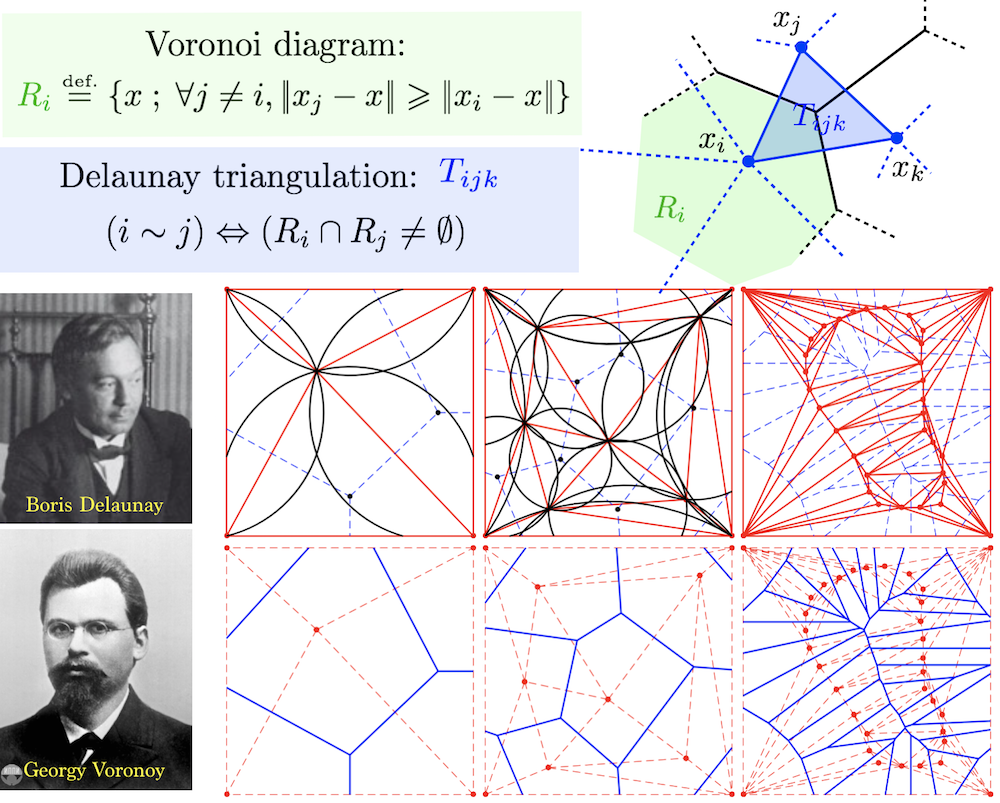
\includegraphics[width=.6\linewidth]{sparse-theory/polytopes/delaunay}
%%
\caption{\label{fig-delaunay}
Visualization of the condition that $\norm{\eta_F}_\infty \leq 1$ as a spherical Delaunay triangulation constraint that all Delaunay spherical caps indexes by identifiable vector should be empty of $(\pm a_i)_i$. 
}
\end{figure}

\begin{rem}[Operator norm]\label{rem-operator-norm}
In the proof, we use the $\ell^p-\ell^q$ matrix operator norm, which is defined as
\eq{
	\norm{B}_{p,q} \eqdef \max \enscond{ \norm{B u}_q }{ \norm{u}_p \leq 1 }.
}
For $p=q$, we denote $\norm{B}_{p} \eqdef \norm{B}_{p,p}$.
%
For $p=2$, $\norm{B}_2$ is the maximum singular value, and one has
\eq{
	\norm{B}_1 = \umax{j} \sum_i |B_{i,j}|
	\qandq
	\norm{B}_\infty = \umax{i} \sum_j |B_{i,j}|.
}
\end{rem}

\begin{thm}\label{thm-support-stable}
	If 
	\eq{
		\norm{\eta_F}_\infty \leq 1
		\qandq 
		\norm{\eta_{F,I^c}}_\infty<1, 
	}
	and $\ker(A_I) = \{0\}$, 
	then there exists $C,C'$ such that if $\max(\norm{w}, \norm{w}/\la) \leq C$, then the solution $x_\la$ of~\eqref{eq-lasso-lagr} is unique, is supported in $I$, and in fact
	\eql{\label{eq-explicit-lownoise}
		x_{\la,I} = x_{0,I} + A_I^+ w - \la (A_I^*A_I)^{-1} \sign(x_{0,I}^\star).
	}
	In particular, $\norm{x_\la-x_0} = O(\norm{w})$.
\end{thm}

\begin{proof}
	In the following we denote $T \eqdef \min_{i \in I} |x_{0,i}|$ the signal level, and $\de \eqdef \norm{A^* w}_\infty$
	which is the natural way to measure the noise amplitude in the sparse setting. 
	%
	We define $s \eqdef \sign(x_0)$, and consider the ``ansatz''~\eqref{eq-explicit-lownoise} and thus define the following candidate solution
	\eql{
		\hat x_{I} \eqdef x_{0,I} + A_I^+ w - \la (A_I^*A_I)^{-1} s_I, 
	}
	and $\hat x_{I^c}=0$. The goal is to show that $\hat x$ is indeed the unique solution of~\eqref{eq-lasso-lagr}. 
	
	
	\noindent\textit{Step 1.}  The first step is to show sign consistency, i.e. that $\sign(\hat x)=s$. This is true if $\norm{x_{0,I}-\hat x_I}_\infty < T$, and is thus implies by
	\eql{\label{eq-supp-stab-proof-1}
		\norm{x_{0,I}-\hat x_I}_\infty \leq K \norm{A_I^* w}_\infty + K \la < T
		\qwhereq
		K \eqdef \norm{(A_I^*A_I)^{-1}}_{\infty}, 
	}
	where we used the fact that $A_I^+ = (A_I^*A_I)^{-1} A_I^*$.
	
	\noindent\textit{Step 2.} The second step is to check the first order condition of Proposition~\ref{sec-prop-uniquness-lagr}, i.e. $\norm{\hat \eta_{I^c}}_\infty < 1$, where $\la \hat \eta = A^* (y-A \hat x)$. This implies indeed that $\hat x$ is the unique solution of~\eqref{eq-lasso-lagr}. One has
	\begin{align*}
		\la \hat \eta &= A^* (A_I x_{0,I} + w - A_I \pa{ x_{0,I} + A_I^+ w - \la (A_I^*A_I)^{-1} s_I ) } \\
			&=  A^* ( A_I A_I^+ - \Id ) w + \la \eta_F.
	\end{align*}
	The condition $\norm{\hat \eta_{I^c}}_\infty < 1$ is thus implied by
	\eql{\label{eq-supp-stab-proof-2}		
		\norm{A_{I^c}^* A_I (A_I^*A_I)^{-1}}_\infty \norm{A_I^* w}_\infty + \norm{A_{I^c}^* w}_\infty + \la \norm{\eta_{F,I^c}}_\infty 
		\leq 
		R \norm{A_I^* w}_\infty - S \la <0
	}	
	\eq{
		R \eqdef K L + 1 
		\qandq
		S \eqdef 1-\norm{\eta_{F,I^c}}_\infty >0
	}
	where we denoted $L \eqdef \norm{A_{I^c}^* A_I}_\infty$, and also we used the hypothesis $\norm{\eta_{F,I^c}}_\infty<1$. 
	
	\noindent\textit{Conclusion.}  Putting~\eqref{eq-supp-stab-proof-1} and~\eqref{eq-supp-stab-proof-2} together shows that $\hat x$ is the unique solution if $(\la,w)$ are such that the two linear inequations are satisfies 
	\eq{
		\Rr = \enscond{
				(\de,\la)}{\de + \la < \frac{T}{K}
				\qandq
				R \de - S \la <0
		}
	}
	This region $\Rr$ is trianglular-shaped, and includes the following ``smaller'' simpler triangle
	\eql{\label{eq-critrion-sign-stability}
		\tilde\Rr = \enscond{
				(\de,\la)}{
				\frac{\de}{\la} < \frac{S}{R}
				\qandq
				\la < \la_{\max} 
		}
		\qwhereq
		\la_{\max} \eqdef \frac{T(KL+1)}{K(R+S)}.
	}
	% A_{I^c}^* ( A_I A_I^+ - \Id ) = A_{I^c}^* A_I (A_I^*A_I)^{-1} A_I^* - A_{I^c}^*
\end{proof}

It is important to realize that Theorem~\ref{thm-support-stable} operates in a ``small noise'' regime, i.e. $\norm{w}$ (and hence $\la$) needs to be small enough for the support to be identifiable (otherwise small amplitude comment of $x_0$ will be killed by the regularization). In contrast, Theorem~\ref{thm-linrate-l1} is ``global'' and holds for any noise level $\norm{w}$. The price to pay is that one has no controls about the support (and one does not even knows whether $x_\la$ is unique) and than the constant involved are more pessimistic. 

A nice feature of this proof is that it gives access to explicit constant, involving the three key parameter $K,L,S$, which controls:
\begin{rs}
	\item $K$ accounts for the conditionning of the operator on the support $I$ ;
	\item $L$ accounts for the worse correlation between atoms inside and outside the support ; 
	\item $S$ accounts for how much the certificates $\eta_F$ is non-degenerate.
\end{rs}
The constant on $\norm{A^* w}/\la$ and on $\la$ are given by~\eqref{eq-critrion-sign-stability}. Choosing (which is in practice impossible, because it requires knowledge about the solution) the smallest possible $\la$ gives $\la = \de \frac{S}{R}$ and in this regime the error is bounded in $\ell^\infty$ (using other error norms would simply leads to using other matrix norm)
\eq{
	\norm{x_0-x_{\la}}_\infty \leq \pa{ 1 + \frac{KL+1}{S} } K \de.
} 

The crux of the analysis of the performance (in term of support stability) of $\ell^1$ regularization is to be able to say wether, for some class of signal $x_0$ of interest, $\eta_F$ is a valid certificate, i.e. $\norm{\eta_F}_\infty \leq 1$. 
%
Figure~\ref{fig-certif-cs} displays numerically what one obtains when $A$ is random. One see that $\eta_F$ is non-degenerate when $P$ is large enough. Section~\ref{sec-cs-certif}�performs a mathematical analysis of this phenomena. 



\begin{figure}
\centering
%%
\begin{tabular}{@{}c@{}c@{}}
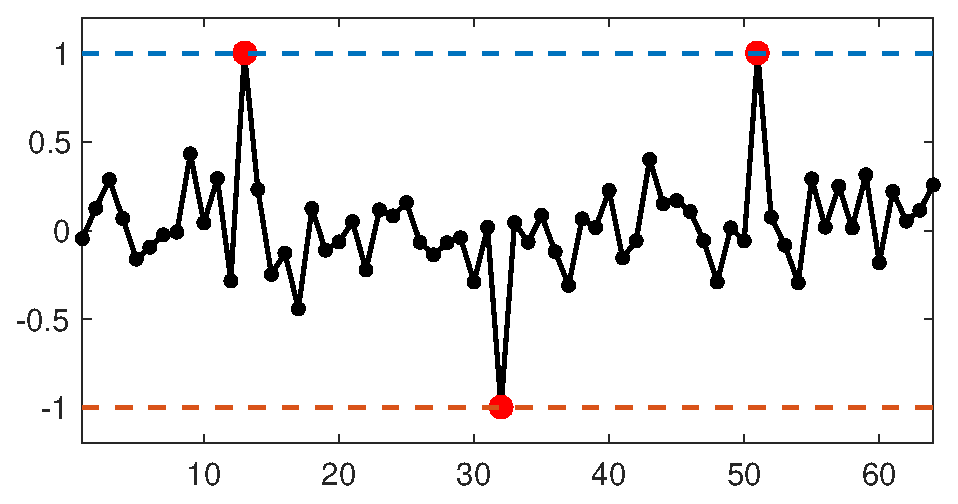
\includegraphics[width=.35\linewidth]{sparse-theory/certificates-cs/certif-cs-64}&
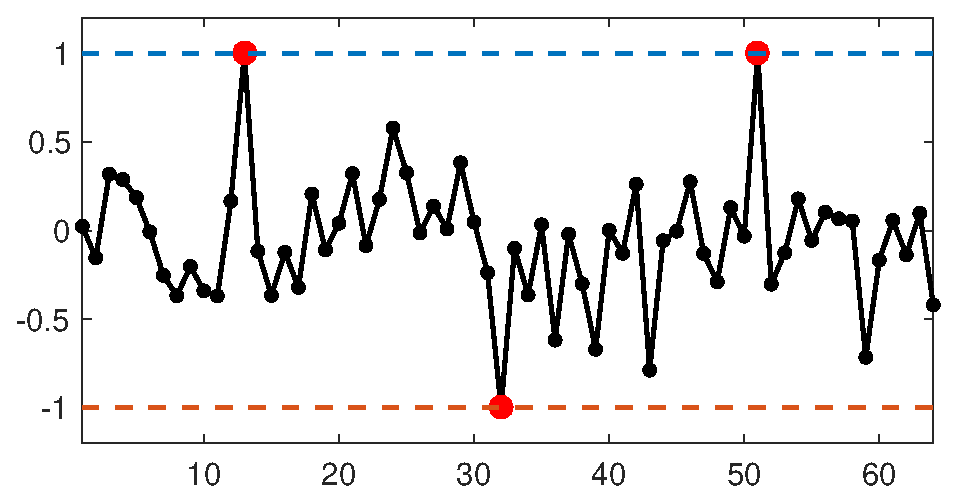
\includegraphics[width=.35\linewidth]{sparse-theory/certificates-cs/certif-cs-32}\\
$P=4$ & $P=8$ \\
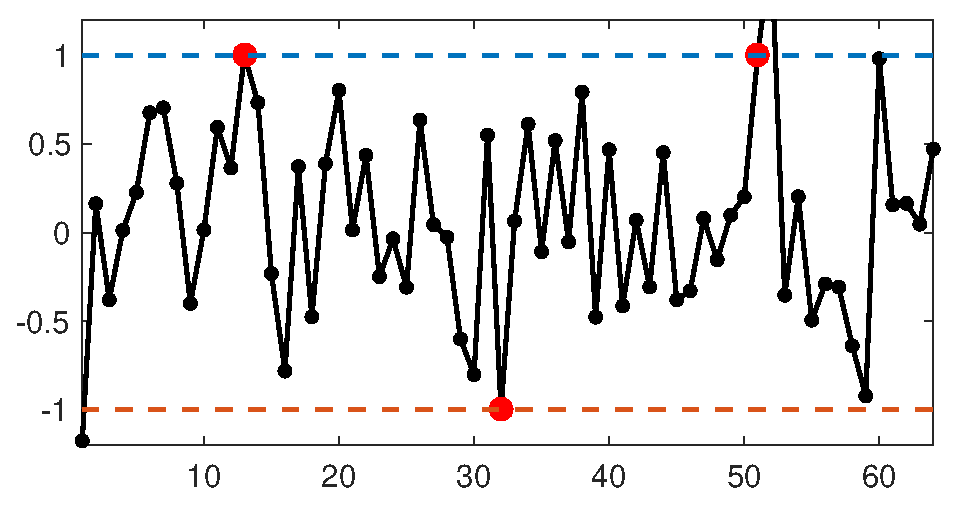
\includegraphics[width=.35\linewidth]{sparse-theory/certificates-cs/certif-cs-16}&
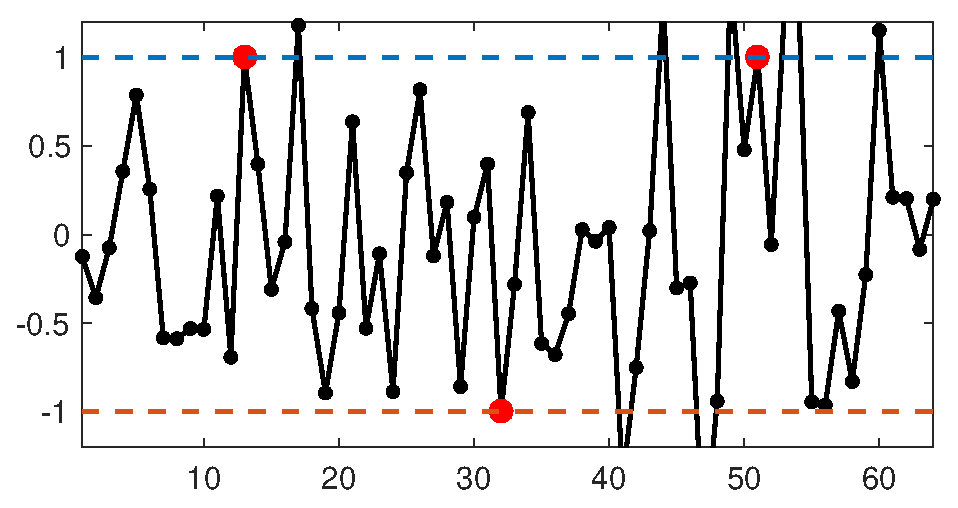
\includegraphics[width=.35\linewidth]{sparse-theory/certificates-cs/certif-cs-8}\\
$P=16$ & $P=32$
\end{tabular}
%%
\caption{\label{fig-certif-cs}
Display of certificate $\eta_F$ for a $A \in \RR^{p \times n}$, $n=64$, with independent Gaussian entries. 
}
\end{figure}

%%%%%%%%%%%%%%%%%%%%%%%%%%%%%%%%%%%%%%%%
%%%%%%%%%%%%%%%%%%%%%%%%%%%%%%%%%%%%%%%%
%%%%%%%%%%%%%%%%%%%%%%%%%%%%%%%%%%%%%%%%
\section{Sparse Deconvolution Case Study}

Chapter~\ref{chap-cs} studies the particular case where $A$ is random, in which case it is possible to make very precise statement about wether $\eta_F$ is a valid certificate.

Another interesting case study, which shows the limitation of this approach, is the case of super-resolution. To simplify the analysis, we assume ``continuous measurement'', and replace the measurement space $\RR^P$ by functions $L^2(\RR^d)$ (for simplicity, we treat here $d=1$). The measurements reads
\eq{
	A x = \sum_{i=1}^N x_i a_i(\cdot) \in L^2(\RR)
}
where the $a_i : \RR \rightarrow \RR$ are smooth functions. A typical example is the deconvolution problem, where $a_i=\phi(\cdot-z_i)$ where $\phi : \RR \rightarrow \RR$ is the smoothing kernel and $(z_i)_{i=1}^N$ is a discretization grid, and for simplicity we assume $x_i=i/N \in [0,1]$.

In this case, this forward model correspond to convolution of measures supported on the grid
\eq{
	A x = \phi \star m_{z,x}
	\qwhereq
	m_{z,x} \eqdef \sum_{i=1}^N x_i \de_{z_i}. 
}

We denote the ``continuous'' covariance
\eq{
	\Cc(z,z') \eqdef \dotp{\phi(\cdot-z)}{\phi(\cdot-z')}_{L^2(\RR)} = \int_\RR \phi(t-z) \phi(t-z) \d t = (\phi\star \bar\phi)(z-z')
}
where $\bar\phi(t)=\phi(-t)$, so that the discrete covariance is $C=(\Cc(z_i,z_i')))_{(i,i')} \in \RR^{N \times N}$ and $C_{I,I}=(\Cc(z_i,z_i')))_{(i,i') \in I^2} \in \RR^{I \times I}$.

Using~\eqref{eq-eta-f-cov}, one sees that $\eta_F$ is obtained as a sampling on the grid of a ``continuous' ' certificate $\tilde\eta_F$
\eq{
	\eta_F = ( \tilde\eta_F(z_i) )_{i=1} \in \RR^N, 
}
\eql{\label{eq-etaf-cont}
	\qwhereq \tilde\eta_F(x) = \sum_{i \in I} b_i \Cc(x,z_i) \qwhereq b_I = C_{I,I}^{-1} \sign(x_{0,I}), 
}
so that $\eta_F$ is a linear combination of $I$ basis functions $(\Cc(x,z_i))_{i \in I}$. 

The question is wether $\norm{\eta_F}_{\ell^\infty} \leq 1$. If the gris is fine enough, i.e. $N$ large enough, this can only hold if $\norm{\tilde\eta_F}_{L^\infty} \leq 1$. The major issue is that $\tilde\eta_F$ is only constrained by construction to interpolate $\sign(x_{0,i})$ are points $z_{0,i}$ for $i \in I$. So nothing prevents $\tilde\eta_F$ to go outside $[-1,1]$ around each interpolation point. Figure~\ref{}�illustrates this fact. 

In order to guarantee this property of ``local'' non-degeneracy around the support, one has to impose on the certificate the additional constraint $\eta'(z_i)=0$ for $i \in I$. This leads to consider a minimum pre-certificate with vanishing derivatives 
\eql{\label{eq-minnorm-certif}
	\eta_V \eqdef A^* p_V
	\qwhereq p_V
	\uargmin{p \in L^2(\RR)} \enscond{\norm{p}_{L^2(\RR)}}{ \tilde\eta(z_I) = \sign(x_{0,I}), \tilde\eta'(z_I) = \zeros_I }.
}
where we denoted $\tilde\eta = \bar\psi \star p$. Similarly to~\eqref{eq-etaf-cont}, this vanishing pre-certificate can be written as a linear combination, but this time of $2|I|$ basis functions
\eq{
	\tilde\eta_V(x) = \sum_{i \in I} b_i \Cc(x,z_i) + c_i \partial_2\Cc(x,z_i), 
}
where $\partial_2\Cc$ is the derivative of $\Cc$ with respect to the second variable, and $(b,c)$ are solution of a $2|I| \times 2|I|$ linear system
\eq{
	\begin{pmatrix} b \\ c \end{pmatrix} 
	= 
	\begin{pmatrix}
		(\Cc(x_i,x_{i'}))_{i,i' \in I^2} & (\partial_2\Cc(x_i,x_{i'}))_{i,i' \in I^2} \\
		(\partial_1\Cc(x_i,x_{i'}))_{i,i' \in I^2} & (\partial_1\partial_2\Cc(x_i,x_{i'}))_{i,i' \in I^2}
	\end{pmatrix}^{-1}
	\begin{pmatrix} \sign(x_{0,I}) \\ \zeros_I \end{pmatrix} .
}
%
The associated continuous pre-certificate is $\tilde\eta_V=\bar\psi \star p_V$, and $\eta_V$ is a sampling on the grid of $\tilde\eta_V$.
%
Figure~\ref{fig-certif-cs}� shows that this pre-certificate $\eta_V$ is much better behaved than $\eta_F$. If $\norm{\eta_V}_\infty \leq 1$, one can apply~\eqref{thm-linrate-l1} and thus obtain a linear convergence rate with respect to the $\ell^2$ norm on the grid. But for very fine grid, since one is interested in sparse solution, the $\ell^2$ norm becomes meaningless (because the $L^2$ norm is not defined on measures). 
%
Since $\eta_V$ is different from $\eta_F$, one cannot directly applies Theorem~\ref{thm-support-stable}: the support is not stable on discrete grids, which is a fundamental property of super-resolution problems (as opposed to compressed sensing problems).
%
The way to recover interesting results is to use and analyze methods without grids. Indeed, after removing the grid, one can show that $\eta_V$ becomes the minimum norm certificate (and is the limit of $\eta_\la$). 




\begin{figure}
\centering
%%
\begin{tabular}{@{}c@{}c@{}}
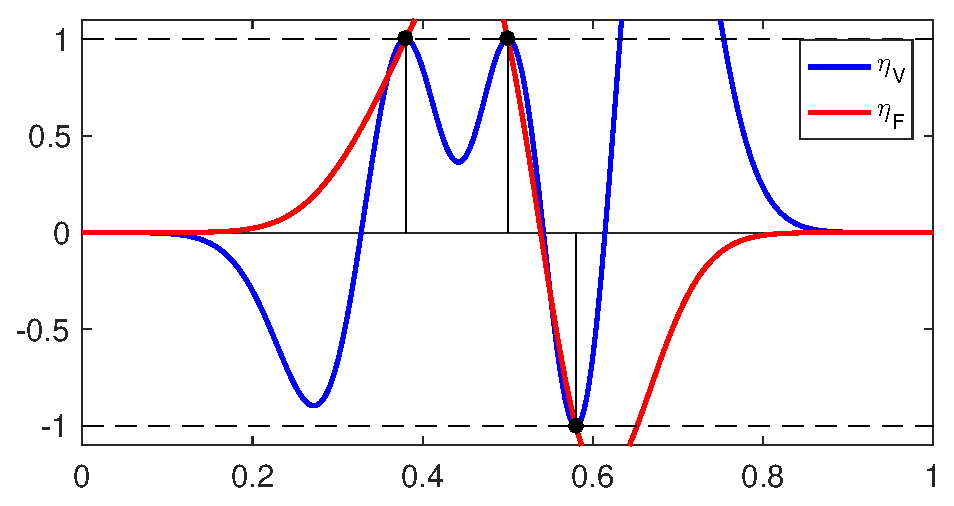
\includegraphics[width=.35\linewidth]{sparse-theory/certif-convol/etaV-N3-d40}&
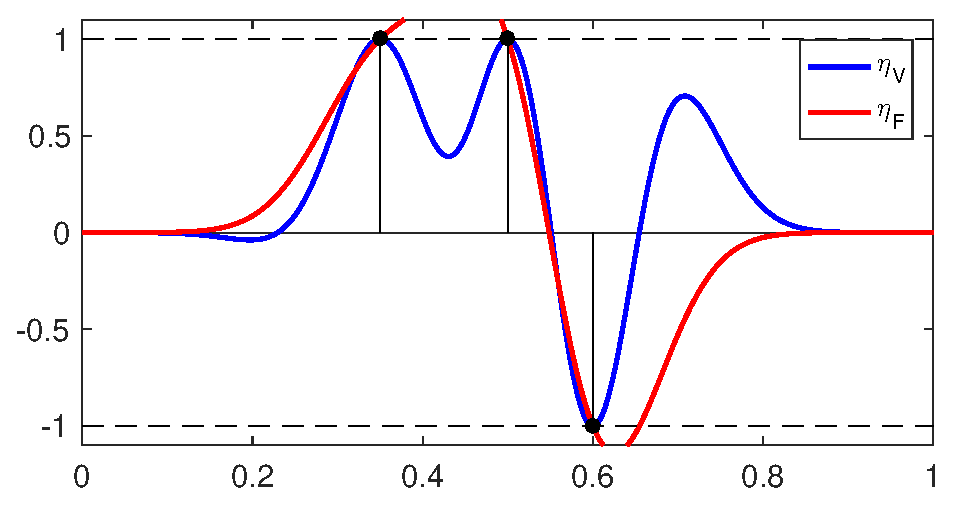
\includegraphics[width=.35\linewidth]{sparse-theory/certif-convol/etaV-N3-d50}\\
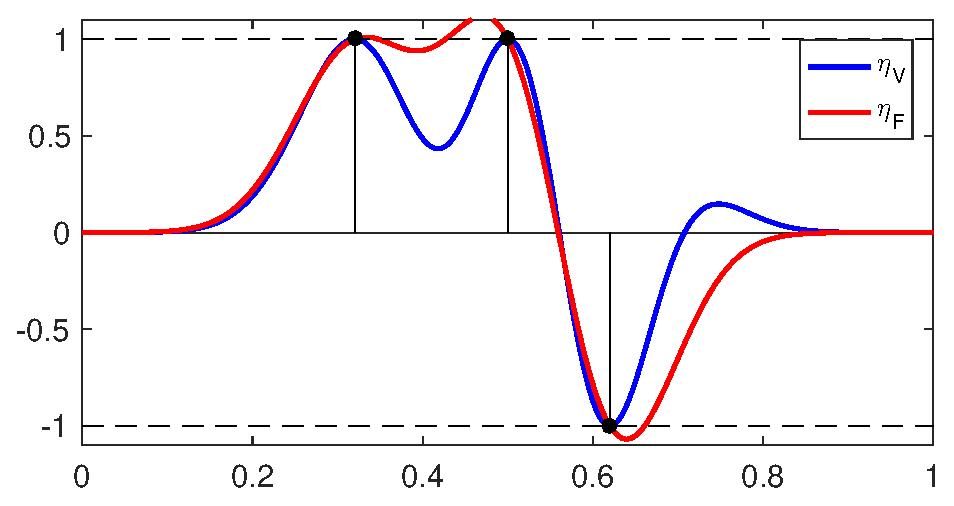
\includegraphics[width=.35\linewidth]{sparse-theory/certif-convol/etaV-N3-d60}&
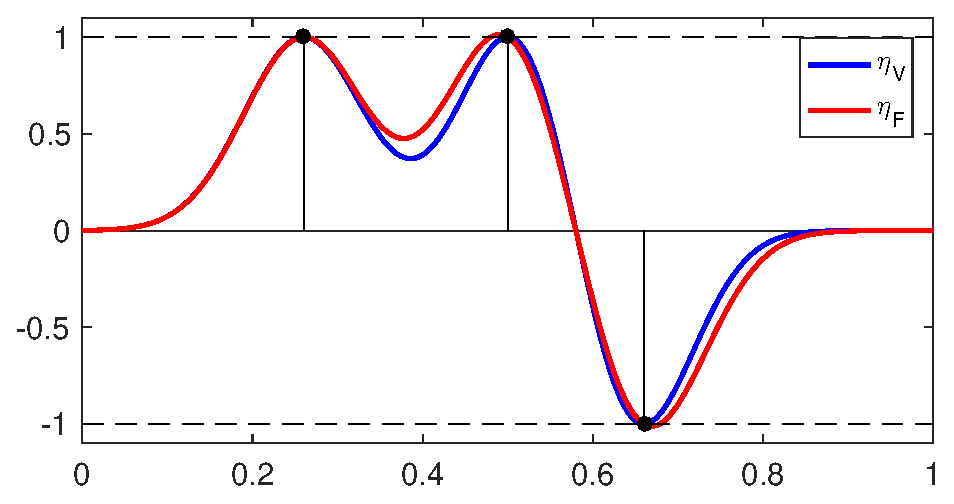
\includegraphics[width=.35\linewidth]{sparse-theory/certif-convol/etaV-N3-d80}
\end{tabular}
%%
\caption{\label{fig-certif-cs}
Display of ``continuous'' certificate $\eta_F$ and $\eta_V$ for $A$ being a convolution operator. 
}
\end{figure}
